\cleardoublepage

\chapter{Estado del Arte de la Domótica}
\label{ch:Capitulo2}

Como definición. el término 'domótica' proviene de la unión de las palabras $domus$ (que significa 'casa' en latín) y $-tica$ (de 'automática', palabra en griego que significa ‘que funciona por sí sola’). Se entiende por domótica al conjunto de sistemas que hacen de una vivienda un edificio inteligente, aportando servicios de gestión energética, seguridad, bienestar y comunicación, y que pueden estar integrados por medio de redes interiores y exteriores de comunicación, cableadas o inalámbricas, y cuyo control goza de cierta ubicuidad, desde dentro y fuera del hogar.


Considerar también las conclusiones de sistemas Centralizados y Descentralizados de este artículo.(\url{http://gritosdetecnologia.blogspot.com/2013/04/origen-de-la-domotica.html})


\section{Politicas de privacidad de marcas con gran presencia de mercado}
\label{ch:Capitulo2.1}

En la descripción de motivaciones del proyecto del capítulo 1, mencionábamos tres marcas que ofrecen suites de domótica a nivel internacional. Todo lo que gira en torno al concepto 'política de privacidad' o 'términos de condiciones de uso', se traduce lamentablemente de forma común, en una aceptación a ciegas de los contratos por parte del usuario final. Esta causa viene motivada generalmente por las complejidades de obtener, abstraer y entender los extensos puntos que conforman estos textos legales, que siguen estando muy lejos de ser amigables. A continuación, observamos como se presentan dichos textos en los siguientes productos de consumo del hogar.

\vspace{1.5cm}

Amazon Alexa (Amazon Movile LLC): Su política de privacidad \url{https://www.amazon.es/gp/help/customer/display.html/?nodeId=GA7E98TJFEJLYSFR} indica que se suben grabaciones del usuario a sus servidores para ser procesadas en sus sistemas de reconocimiento de voz y compresión de lenguaje. No se indica expresamente que dichas grabaciones además son incluidas en procesos de entrenamiento de machine learning para mejorar su aplicación. Se indica además que su dispositivo no graba continuamente, salvo por reconocimiento del comando de activación (generalmente el nombre del dispositivo), pero tampoco se especifica cuanto tiempo graba, ni que hace con las filtraciones de voz de otras personas que estén presentes. La cláusula de servicios a terceros resulta bastante ambigua, pero indica que cualquier cesión de permisos a una aplicación de terceros que se integre con Amazon, podrá requerir datos a la misma. Se pueden encontrar más detalles en sus condiciones de uso \url{https://www.amazon.es/gp/help/customer/display.html?nodeId=201809740}, en la misma, podemos observar adicionales clausulas anidadas que redirigen a nuevos enlaces como las condiciones de uso de Amazon España \url{https://www.amazon.es/gp/help/customer/display.html?nodeId=200545940}. Al final es realmente difícil saber a qué se atiene un usuario que adquiere este producto. Su aplicación de movil también requiere un abanico realmente extenso de permisos en el SO de un Smartphone/tablet, incluyendo gestión de cuentas en el dispositivo (añadir o eliminar cuentas), accesos a contactos, ubicación, mensajería, llamadas, almacenamientos, dispositivos de entrada/salida y un largo etcétera que puede consultarse en la APP store correspondiente de Android/IOs.

\vspace{1.5cm}

GoogleHome (Google LLc.): Google lleva años intentando mejorar su calidad de servicio respecto a las leyes europeas de protección de datos. Aun habiendo sonados casos de tratamiento ilegal de DCPs que han terminado en sanciones a la compañía, como los de la AEPD impuestas de hasta 900.000 euros \href{https://www.abc.es/tecnologia/redes/20131219/abci-google-multa-aepd-201312191217.html}{noticia de ABC}, eso no ha impedido la expansión de la compañía a lo largo del mundo. todo ello condicionado por su presencia internacional, que en algunos países son además, proveedores de servicios e infraestructuras de instituciones públicas como ocurre en la Universidad Complutense de Madrid, asi como proyectos conjuntos como la \href{https://biblioteca.ucm.es/google8}{digitalización de la biblioteca complutense}.En el campo de la domótica, lo que respecta a su política de privacidad en su aplicación Google Home, se remite al usuario a las \href{https://policies.google.com/privacy?hl=es}{condiciones generales} de la compañía de Google LLc, para información más concreta sobre $Google Home$ es necesario buscar información concreta en la \href{https://support.google.com/googlehome/answer/7072285?hl=es&ref_topic=7173611}{página de ayuda de Google}. En las misma se afirma la intención de recoger datos (no se especifican de que naturaleza), con el fin de usarse en $machine learning$, afirman que podrían existir aplicaciones de terceros que nutran a Google con más datos (tampoco se especifican que datos ni que aplicaciones de terceros). Aun asi, ofertan la posibilidad de gestionar los datos almacenados por Google en su \href{https://myactivity.google.com/}{gestor de actividad} y en caso de tener la configuración por defecto de recogida de datos que Google utiliza en los SO de Android, los resultados son como poco inquietantes. Un sistema de domótica de Google es perfectamente capaz de determinar con exactitud casi toda tu vida diaria en casa, incluyendo cuando has dormido, cuando has comido, que cosas has visto y que actividades has desarrollado.

\vspace{1.5cm}

Xiaomi Mi (Xiaomi INc.): La empresa china que ha irrumpido en el mercado europeo gracias a sus aplicaciones con UX amigables y precios de dispositivos competitivos, que además admiten múltiples de dispositivos clónicos de fabricantes no adscritos a la marca de Xiaomi. También está haciendo sus adaptaciones para operar en Europa bajo el marco de la RDPG, su \href{https://www.mi.com/es/about/privacy}{política de privacidad}, sobre la recopilación de datos es cuanto menos, ambigua, usando frases como, "podemos recopilar la totalidad o una de la parte que usted nos proporciona" , y en lo que respecta a de que manera se utiliza dicha información, es tan extensa que solo remarcaremos que aparece el nombre de la compañía Facebook en uno de los puntos. Se afirman en que no se venderán los DPCs a terceros salvo aceptación del usuario. La estrategia de la compañía de Xiaomi en su aplicación pasa por ofertar toda clase de servicios, incluyendo chats, foros, pagos en la plataforma de AliPay, etc. La consecuencia de estos servicios genera la tabla más larga de permisos necesarios en un smarthpone/tablet de los ejemplos mencionados. Definitivamente, aquel usuario que instale esta aplicación y permita a todos esos permisos ya puede olvidarse de su privacidad.

\section{Frameworks disponibles para la gestión de IoT para SmartHomes}
\label{ch:Capitulo2.2}

Un planteamiento recurrente en el diseño de una solución basada en software es acelerar el proceso de desarrollo e implementación utilizando un framework. Es una buena idea. Estas herramientas están, en su mayoría, profundamente documentadas para exprimir sus capacidades al máximo, disponen de versionados y revisiones (en mayor o menor medida) que fortalecen tanto su seguridad, robustez, resiliencia e implementación. Poseen una buena abstracción del hardware en el que se ejecutan, sus servicios son modulares, su arquitectura es escalable.  En ocasiones están basados en software libre y/o gratuito, y disponen de una comunidad activa de usuarios a los que poder preguntar dudas. Estas son cualidades muy importantes, mas alla de las capacidades técnicas que cada opción pueda ofrecer.
En el mundo del IoT es impórtate determinar el alcance en conectividad que se desea alcanzar y volumen de datos a tratar. Existen frameworks pensados para interconectar ingentes cantidades de dispositivos en grandes extensiones de terreno y bajo el peso de un abrumador volumen de datos que procesar como es el caso de las SmartCities, o la infraestructura del sector primario y secundario. En algunos casos, el alcance es tan extremo que el concepto de IoT evoluciona a IoE (Internet of Everything) y se requiere la presencia de grandes actores tecnológicos, y sus soluciones, para abarcar estos proyectos, como es el caso del framework IBM BlueMix de IBM, el Cisco Virtualized Packet Core de Cisco, AWS IoT de Amazon o Azure IoT de Miscrosoft, por mencionar algunos ejemplos de este calibre.

\vspace{1.5cm}

Evidentemente, estos frameworks no fueron diseñados pensando en reducidos entornos como los de un hogar, y aunque son compatibles, el tiempo necesario en formación para su uso queda fuera de las capacidades y expectativas de un proyecto de las características que aqui se recoge. Sin embargo, también se dispone de un amplio abanico de opciones a un alcance más acorde a lo esperado de una solución SmartHome.

\vspace{1.5cm}

Existe una serie de criterios que aplicaremos al valorar las opciones de frameworks disponibles, en consonancia con la motivación de este proyecto. Antes de realizar cualquier evaluación sobre las bondades de cada plataforma, es conveniente recordar que en la solución que esperamos crear, se intentara evitar el uso de servicios en la nube o dependencias de APIs externas. Esto responde al objetivo de aislar la suite domótica a desarrollar, de la red de internet, evitando esa dependencia para su operatividad. Por supuesto, no es el objetivo crear una plataforma desconectada, ya que, se espera poder operar de forma remota los dispositivos desde fuera del ámbito de la red local del hogar. Ademas, debera disponer de un licenciamiento de codigo libre y gratuito, en otro caso, estariamos contraviniendo la naturaleza de este proyecto.

\vspace{1.5cm}

FiWare esta catalogada como una plataforma de codigo abierto que agrupan un set de estandares universales para el contexto de gestion de datos~\cite{whatisfiware}. Se sustenta en la ejecución del framework sobre Dockers que pueden ser alojados localmente en maquinas dentro del hogar, y aunque esta solución esta orientada a procesar datos en un contexto mas extenso que una SmartHome, puede aislarse de la red de internet. Limitan la portabilidad de las aplicaciones a aquellas que se catalogen como 'Powered by FIWARE', y aunque ofrecen una interfaz estandar para los componentes que integren la solución, con el objetivo de eliminar el bloqueo del proveedor de componentes, no posee un licenciamiento de codigo libre, por ello sera descartado.

\vspace{1.5cm}

OpenHab es otro nombre que es recomendado frecuentemente en foros y ponencias de IoT, bajo el nombre de 'Open Home Automation Bus', esta plataforma dispone de manuales de instalación para convertir un ordenador en un centro de control de domótica, incluyendo la propia Raspberry Pi con una imagen preconfigurada~\cite{openHabRaspberryPi}. La documentación detalla la definición de un modelo de desarrollo orientado a objetos flexible y escalable, donde las 'things' representan a los dispositivos físicos, que incluyen las propiedades para gestionar sus canales de comunicación a 'items' que representan la capacidades y propiedades de los automatismos del hogar. También se proponen reglas, que definen comportamientos en función de los disparadores asignados por el usuario. De esta forma, puede automatizarse el apagado de las luces de una estancia si en esta no hay individuos. Dispone de un extenso abanico de interfaces, incluyendo un chatbot llamado HABot para controlar la suite domótica con un lenguaje natural escrito, esta función, por ejemplo, ha sido objeto de proyecto en un reciente trabajo de fin de master de la facultad de informática~\cite{eprint49443}. Posee REST API que permite una Inter operatividad con servicios externos o desarrollos propios y soporte para todas las principales plataformas móviles (Android, IOs, Windows) ya que está programado en Java. No se limita tampoco en interoperatividad de buena parte de servicios y stacks de desarrollo existentes, y dispone de una extensa gama de dispositivos compatibles mediante Add-ons, como, por ejemplo, Chromecast o philips Hue, otras soluciones domóticas como ‘Max! Home Solutión’, o protocolos como MQTT o estándares de redes con TCP/UDP o WOL (Wake on LAN) entre otros. De hecho, salvando que su licenciamiento se limita a ser open source, es de lejos, una de las mejores opciones disponibles que cumplen con lo necesario para crear una solución domótica aislada, ya que, no genera dependencias de servicios externos, puede ser operada localmente o de forma remota y dispone de capacidad suficiente en cuanto a soluciones modulares para cubrir los futuros casos de uso que se plantearan. Open Hab esta en sintonia de los objetivos de este documento, cubre las necesidades de nuestro alcance y mucho mas. De hecho, cubre tantas posibilidades y entregan tanto trabajo pre-maquetado y listo para ejecutar, que en las primeras pruebas nos sentimos totalmente vacios. Perdimos la capacidad de experimentar los distintos niveles que conforman una suite domótica, por que este framework ya lo proporcionaba practicamente todo. Ademas, su documentación es bastatne extensa, y al no estar seguros de absorberia nuestro tiempo de analisis de otras opciones, decidimos no implementarlo,

\vspace{1.5cm}

En el proceso de estudio de diversos frameworks encontramos otras opciones. En realidad el abanico de soluciones disponibles es muy extenso,

\begin{itemize}
\item thingsboard
\item Pimatic
\item Calaos: Home automation solution and a complete distro
\item Domoticz
\item Home Asistant: Home automation platform running on Python 3
\item OpenMotics : Complete home automation platform
\item Jeedom
\item MisterHouse: Supports X10, voice recognition and several serial devices
\end{itemize}

Ya que uno de los objetivos del proyecto radica en la condición de disponer de una licencia libre, nuestra investigación nos ha llevado a conocer MainFlux. Se cataloga como una plataforma tecnológica de codigo abierto y patente libre con licencia Apache 2..0. Incluso ofrece un dispositivo gateway para soluciones industriales y de computación desarrollada por la misma Linux Foundatión. Esta planteado como PaaS para integrar aplicaciones que interactúan con los dispositivos de la SmartHome mediante un gateway. La plataforma, dispone de una versión gratuita para ser alojado localmente en un Docker o un equipo con SO Linux. Su documentación clarifica que el desarrollo de aplicaciones que conectaran a Mainflux se realizaran a través de protocolos bridging (como HTTP, MQTT,WebSocket, CoAP)~\cite{mainfluxdoc}.


Sin frameworks, aunque supone un mayor esfuerzo, puede orientarse mas concreteamente a nuestros objetivos mas cercanos.

\section{Stack de servicios, estandares  protocolos de comunicación}
\label{ch:Capitulo2.3}

Orientando la selección de los servicios necesarios para la creación de un prototipo, que permita alcanzar los objetivos planteados para este proyecto, surge la necesidad de disponer de un servicio de infraestructura web, que permita gestionar la suite domótica cómodamente desde un dispositivo remoto. Sin entrar en definiciones, nos centraremos en que características que mejor se adapten a las necesidades del proyecto.

\vspace{1.5cm}

Para nuestra estrategia de selección de servicios, empezaremos seleccionando la BBDD que cimentaran el resto de stack. Toda aplicación informática, se sustenta en primera instancia sobre el almacenamiento de datos de manera persistente. En esencia, las BBDD se segmentan en 2 categorías principales según como se relacionan entre si dichos datos. Estos son, BBDD relacionales, o BBDD no relacionales. Además de esta segmentación principal, existen otras características remarcables en cuanto a la escalabilidad y diseño de cada modelo. Si consideramos como, humanamente, entendemos los datos necesarios para una suite domótica, una de las primeras impresiones, es que no sabemos con certeza cuantos dispositivos de sensorización o actuadores serán necesarios para cada caso de uso. De hecho, es muy probable que un mismo caso de uso disponga de diferentes combinaciones de dispositivos para alcanzar una solución. Es, sin embargo, bastante obvio que básicamente almacenaremos pocos conceptos primarios, los principales son, ubicaciones, dispositivos en las ubicaciones y medidas y/o acciones de los dispositivos.

\vspace{1.5cm}

Podría parecer que hablamos de una relación de objetos entre sí, y que un modelo de BBDD relacional es la mejor opción, pero si consideramos que, cada entrada almacenada tendrá una estructura distinta, hace que no sea una opción tan ideal. Pensemos, por ejemplo, que utilizando una BBDD SQL se planifica un conjunto de tablas relacionadas entre sí. Sera necesaria una tabla que contenga las ubicaciones y se relacione con otra tabla que definan a los dispositivos. Esto establece una relación 1:N donde múltiples dispositivos pueden existir para una estancia, pero nunca en varias a la vez. De cada dispositivo existirá una nueva relación 1:N de medidas. Lo cual deja un esquema semejante al de la figura siguiente:


\begin{figure}[hbt!]
\centering
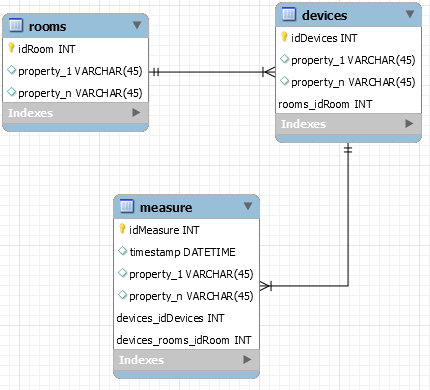
\includegraphics[height=2.5in]{figures/SQLSchemaExample_1.png}
\end{figure}

\vspace{1.5cm}

Sin embargo, existen algunos problemas graves de diseño de esta idea, en primer lugar, los dispositivos no pueden ser una propiedad de una estancia. Son objetos relacionados, pero no existe una transitividad dura entre ellos. Un dispositivo puede cambiar de estancia en un momento dado, y aun asi, seguir existiendo medidas en fechas concretas de ese dispositivo para una habitación en la cual, dicho dispositivo ya no está relacionado. Otro posible escenario es la desaparición de una estancia (como resultado de fusionar 2 estancias en una al derribar una pared). Para mantener una integridad lógica y persistente a lo largo del tiempo. Toda medida deberá tener un campo que determine en que ubicación fue tomada.
no hay transitividad dura entre room y device, lo cual hace que sean independientes entre sí.


\begin{figure}[hbt!]
\centering
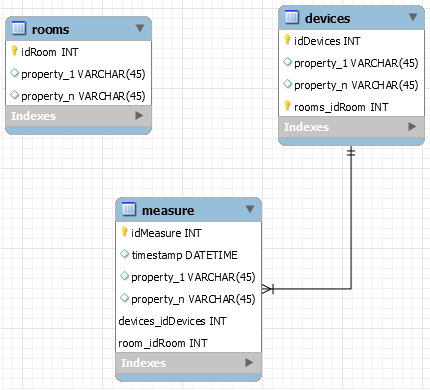
\includegraphics[height=2.5in]{figures/SQLSchemaExample_2.png}
\end{figure}

\vspace{1.5cm}

Con esto aún tendríamos que enfrentar un problema adicional, el número de columnas que definen las propiedades de una tabla. El ejemplo más claro es la tabla de medidas. Una medida, efectuada por un sensor será definida por su identificador y la fecha en la que se realizó, ahora bien, según la naturaleza del dispositivo, se obtendrán disantos tiempos de medida. Un sensor combinado de temperatura y humedad nos dará dos magnitudes de medición, un sensor de ruido almacenará un valor de decibelios, una luz define su medida por su estado de actividad (encendido o apagado), aunque por otra parte podría indicar el consumo eléctrico, o propiedades adicionales como intensidad de luz, o incluso color. Es cierto que, para un actuador, como lo es un emisor de luz, no realiza medidas como tal, y sus correspondientes estados de actividad podrían ser más adecuados definirlos como propiedades del dispositivo y no como medidas. Podríamos separar las medidas de los estados en tablas distintas, pero igualmente llegaríamos al problema del número de campos necesarios en una tabla. Valor que por otra parte es muy difícil de prever en base a la extensa gama de dispositivos existentes. Esto puede solucionarse de manera sencilla con 2 estrategias. Incluir una gran cantidad de columnas en previsión de los distritos tipos de medidas existentes, dejando que las medidas posean un valor nulo para los campos no utilizados en función de la relación de su sensor, o bien, unificar todos los campos en un único valor de cadena de caracteres que almacene un dato estructurado, como es el caso de los JSON. Esta última opción, sería la más deseable tanto por sencillez de implementación como facilidad de procesamiento. Lo que dejaría un esquema semejante a este:

\begin{figure}[hbt!]
\centering
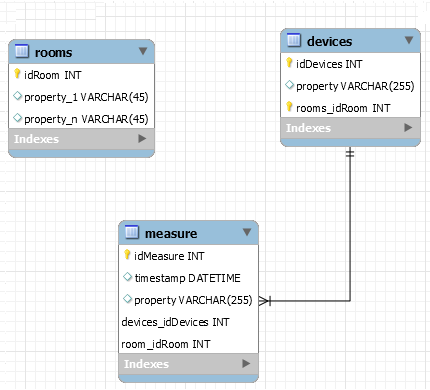
\includegraphics[height=2.5in]{figures/SQLSchemaExample_3.png}
\end{figure}

Una preocupación que agrava la perspectiva de usar una BBDD relacional es, en este punto del proyecto, su escalabilidad horizontal. Si bien las tablas pueden crecer a un gran número de registros, no se prevé almacenar datos con vistas a largo plazo, la mayoría de los valores almacenados serán efímeros en tiempo de utilidad, almacenarlos responde solo a la necesidad de obtener comparativas en plazos de tiempo relativamente cortos, como horas, dias, y posiblemente semanas. Mas alla de este rango estos datos no tienen una utilidad real y pueden ser condensados en médias para utilizarse en resúmenes. Por otro lado, disponer de flexibilidad a la hora de configurar la extensión de propiedades de un objeto de la BBDD es uno de los puntos fuertes de una BBDD no relacional.

\vspace{1.5cm}

En la mayoria de proyectos de IoT observados en nuestras indagaciones, aparece en escena mongoDB. Es una elección popular gracias a su escalabilidad y flexibilidad, esto permite sortear mas facilmente la problematica de adaptarse y anticiparse a los cambios tan continuos que sufre el escenario del IoT. Aparecen nuevos sensores continuamente, que generan nuevas muestras de datos, con funcionalidad deistitnas, en una BBDD relacional es dificil realizar iteraciones del modelo de datos de esta manera. Por otro lado, el proceso de analizar unos datos que evolucionan continuamente, no solo en contenido, sino en forma, hacen que su extracción y procesado se vuelva muy compleja. Las BBDD no relacionales son mas amigables a la hora de definir criterios para extraer informaciones concisas dentro de un documento heterogeneo. Ademas, MongoDB esta pensado para trabajar estrechamente con datos presentados en formato JSON. Esto hace su uso muy conveniente en un entorno de aplicación que se base en estas estructuras de datos como ocurre con los motores de JavaScript de los navegadores o la mayoría de aplicaciones moviles.

\vspace{1.5cm}

Destacar este ultimo aspecto es determinante a la hora de seleccionar el entorno de ejecución que usara el servidor de la aplicación de domótica. En este aspecto, existen multiples estrategias, todas ellas en una primera aproximación valdias. Se puede disponer de un servidor web como Apache o Ngix, programados en lenguaje PHP. El cliente establece conexiones por el protocolo HTTP/HTTPS solicitando procesamientos por aprte del servidor y este entrega una respuesta codificada en texto plano para que el sotware del cliente lo reciba. Esta estrategía es simple pero efectiva, sin embargo, en proyectos de IoT, hay un protocolo originalmente ideado por la compañia de IBM de licencia libre enfocado a una conectividad maquina a maquina (M2M), el código de dicho protocolo fue donado en 2011 al proyecto de Eclipse. Mientras que el protocolo HTTP/HTTPS puede manejar volumenes grandes de información en su trasferencia por la red de comunicaciónes, el protocolo MQTT requiere menos ancho de banda, esta orientado a proyectos con un bajo consumo  y que dispongan de poco recursos de procesamiento. Sin perder de vista el objetivo principal de conseguir en una suite domotica, por ejemplo, si hay que obtener la temperatura de una habitación, todo se reduce a un unico dato, un numero (posiblemente decimal), o al menos, eso es lo que un usuario espera recibir. Esto implica que, un sensor de temperatura, en algun lugar de la casa, recibe una petición en la red en la que se encuentra de otro dispositivo, toma la medida y la envia a dicho dispositivo.

\vspace{1.5cm}

Si usamos el planteamiento de un servicio web, el sensor dispondrá de la capacidad de recibir una solicitud en un puerto abierto, cuando reciba la petición adecuada, respondera incluyendo en el cuerpo de la respuesta dicha medida y sera procesada en el dispositivo que creó la petición. Esto significa que cada sensor/actuador sera por si mismo un servidor web con un puerto abierto que atiende peticiones de clientes. Si todos los dispositivos estan conectados en la misma red, salvo que se apliquen restrinciones especificas en el firewall, seran visibles entre si, pudiendo encadenar llamadas y respuestas entre ellos, o a traves de un dispositivo central que se encarge de hacer las solicitudes y cuyas respuestas recibidas sean procesadas para mostrarse en la aplicación movil.

 -- OJO
 un servicio web puede ser caro para un arduino. Hay papers sobre el consumo energético de servicios web vs mqtt

Desde el planteamiento del protocolo MQTT, la estrategia gira en torno al concepto de sucripción de $topics$ o temas, donde los dispositivos publican información de distintos temas y los suscriptiores a dichos temas reciben la información cuando es publicada. A nivel físico, todos los clientes se conectan a un punto central, lo que define una topología de estrella (con sus ventajas e incovenientes). Dicho nodo central es el servidor definido como $broker$, y es el unico que sabe a que topic esta suscrito cada cliente. Esto significa que cada uno de los sensores/actuadores de la red ignora al resto de los dispositvos, ya que solo atienden la comunicación con el broker a traves de una conexion TCP permanente. Esta estrategia es diferente a la usada en el protocolo HTTP, ya que no es necesario hacer una petición para recibir información de un cliente. Simplemente el broker da o solicita información en los topics a los que los dispositivos estan suscritos. Para proyectos de este tipo, el hecho de que los dispositivos no se relacionen entre si, dan lugar a una gran ventaja, la escalabilidad.

\vspace{1.5cm}

La escalabilidad de una suite domótica es un factor determinanate al considerar su implementación. Que los dispositivos que conforman la red puedan cambiar con facilidad su organización, numero o capacidades son un valor añadido.

-- Resta hablar de Angular y NODE

-- encajar por aqui esto:

La domótica se remonta a los años 70, uno de los primeros hitos fue el \href{https://es.wikipedia.org/wiki/X10}{protocolo de comunicaciones X-10}~\cite{x10protocolwikipedia} de automatización de dispositivos en la línea eléctrica de un hogar. Con él, se puede utilizar la propia red como canal de comunicaciones mediante ráfagas de pulsos. El ancho de banda de 256 dispositivos simultáneos es una cantidad más que suficiente para interactuar con los dispositivos de un hogar, si calculamos que cada elemento susceptible de ser automatizado como por ejemplo persianas, estufas, enchufes, e interruptores ocupase un espacio de este ancho de banda, seguirían sobrando espacios en un piso de 150 metros cuadrados

\vspace{1.5cm}

En pleno 2019 pueden adquirirse los dispositivos necesarios para instalar una red X-10 que incluye interruptores, actuadores, sensores, transmisores, interfaces y unidades de control (todos ellos necesarios para obtener el control completo de la red) por precios con rangos entre 20 a 70 euros por cada elemento. Esto supone inversión elevada si se tiene en cuenta un hogar de varias habitaciones. Hay que considerar además ciertas limitaciones como que cada controlador es capaz de manejar un número limitado de dispositivos.

\vspace{1.5cm}

En cuanto a las aplicaciones necesarias para gestionar el sistema, X-10 posee alternativas de código libre para su desarrollo como \href{http://www.minervahome.net/}{Minerva}. También existen interfaces hardware que traducen el protocolo X-10 a APIs de servicios web como el dispositivo \href{http://www.iobridge.com/}{ioBridge} que supuso una disrupción en el ámbito del IoT y la automatización del hogar.

\vspace{1.5cm}

El problema de la solución del X-10 no radica en su protocolo sino en los costes, que generalmente sobrepasan los cientos de euros para las configuraciones mas sencillas. Además, esta instalación requiere de un proceso de obra, ya que es necesario empalmar los componente a la red eléctrica del hogar. En realidad, la opción de usar dispositivos del protocolo X-10 esta condicionada a que la red eléctrica del hogar se instalara durante el proceso de edificación con vistas a utilizar este sistema. De otra forma, sera necesario planificar obras y esto complica la facilidad de crear un prototipo asequible.

\vspace{1.5cm}

Una década después surgiría el SCE (Sistema de Cableado Estructurado) que permitía el trasporte de datos y voz, esto supuso la aparición del concepto Edificio Inteligente. Sin embargo, esto requiera de una instalación compleja difícilmente viable en edificios ya existentes, como es el caso que ocupa el alcance de este proyecto. Con la aparición de las redes inalámbricas, y sus posteriores estándares de comunicación como el WIFI, se popularizaron los sistemas de domótica aplicada directamente sobre los dispositivos, sin tener en cuenta la red eléctrica que los hace funcionar.

zigbee
\begin{figure}[hbt!]
\centering
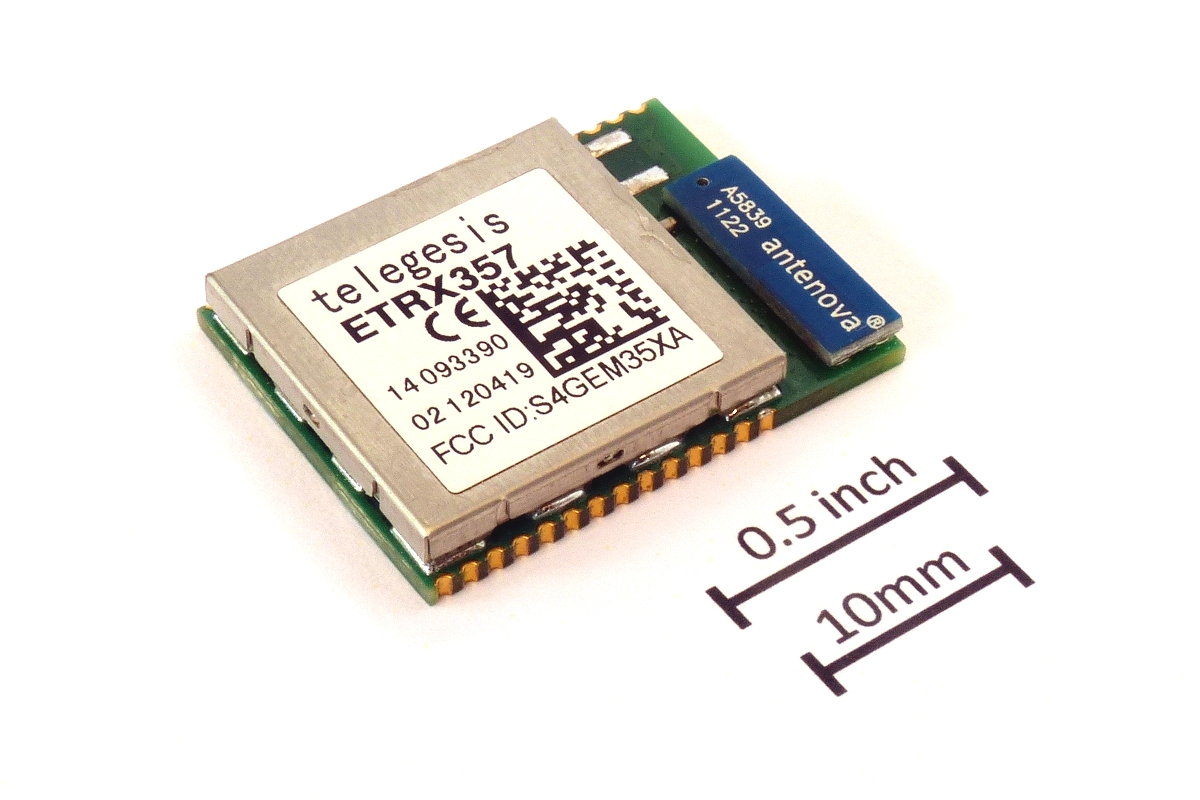
\includegraphics[height=2.5in]{figures/ETRX357_ZigBee_module_with_size_ref.jpg}
\caption[captura de una Raspberry]{Ordenador Raspberry Pi 3B\footnotemark}
\end{figure}



\section{Hardware disponible}
\label{ch:Capitulo2.4}

Se han descrito algunas de las tecnologías características de las aplicaciones, topologías de red y protocolos de comunicación utilizados en domótica. Pero todo este entramado de software y señales deben operar en hardware físico. Mas concretamente en múltiples dispositivos de hardware. En \gls{iot} el abanico de fabricantes de dispositivos orientados a sensorización y actuadores es tan extenso que simplemente esta fuera de todo alcance el enumerarlos en este documento, aun así, considerando los objetivos definidos en el proyecto, que incluyen el uso de hardware open source, y costes de adquisición reducidos, podemos reducir una lista de opciones acotada.

\vspace{1.5cm}

Es importante remarcar en este punto del documento, que en los proyectos de \gls{iot}, obtener el mejor balance de coste y eficiencia en la construcción es vital para soluciones profesionales. Para el prototipo que ocupa este proyecto, no se espera enfrentar este obstáculo, ya que, no se encuentra definido en los objetivos, el crear un sistema los mas equilibrado posible, sino uno funcional, respetando un limite de gasto que no supere la cuantía definida de 50 euros. Tampoco figura entre los objetivos asegurar un consumo energético los mas reducido posible por aparte de los dispositivos, pero se valorará la selección de equipamiento que, dando la mayor flexibilidad de configuración, se encuentre en valores de consumo lo suficientemente bajos como para que el prototipo sea fiable al ideal de una suite domótica funcional.

\vspace{1.5cm}

Partimos del concepto de suite domótica basado en dispositivos conectados a un nodo principal o gateway, el cual actúa como router wifi. Dicho gateway posee un adaptador de red adicional que permite una conexión con la red de internet y que sea capaz de ejecutar servicios y aplicaciones actuando como servidor. Estos requisitos nos orientan a disponer de un ordenador completo, sera necesaria la flexibilidad de un SO que nos permita experimentar diferentes planteamientos, sin dejar de tener es cuenta que este ordenador tendrá una disponibilidad continua, y debe tener un consumo energético bajo y unos recursos suficientes para actuar como cimiento del prototipo.

\vspace{1.5cm}

Hace una década habría sido necesario apuntar a un equipo muy especializado y esto generalmente se traduce en un incremento del precio del equipo. Hoy, en cambio, disponemos de muchas opciones de ordenadores con un reducido factor de forma, bajo consumo eléctrico y recursos mas que suficiente para cubrir muchos prototipos ligueros. Hablamos de la muy conocida Raspberry Pi y similares que has surgido con el tiempo (como Orange Pi, Banana Pi, Odroid o Matrix ARM ~\cite{lignuxComparative}), pueden encontrase en la figura \footnotetext{Comparativas de micro-ordenadores} algunos aspectos técnicos de sus capacidades comparadas entre si.
. Para el caso que nos ocupa necesitamos que disponga de al menos dos adaptares de red, uno de ellos inalámbricos, aunque puede subsanarse la falta del mismo mediante adaptadores inalámbricos USB (una estrategia muy común en los primeros modelos de Raspberry Pi hasta la serie 3). No es necesario que disponga de un procesador gráfico ya que operaremos de forma remota el ordenador mediante conexiones de SSH. Sera un aspecto muy positivo que disponga de una interfaz para conectar dispositivos USB, este ultimo responde a la posible necesidad de conectar placas micro-controladoras para su programación.

\begin{figure}[hbt!]
\centering
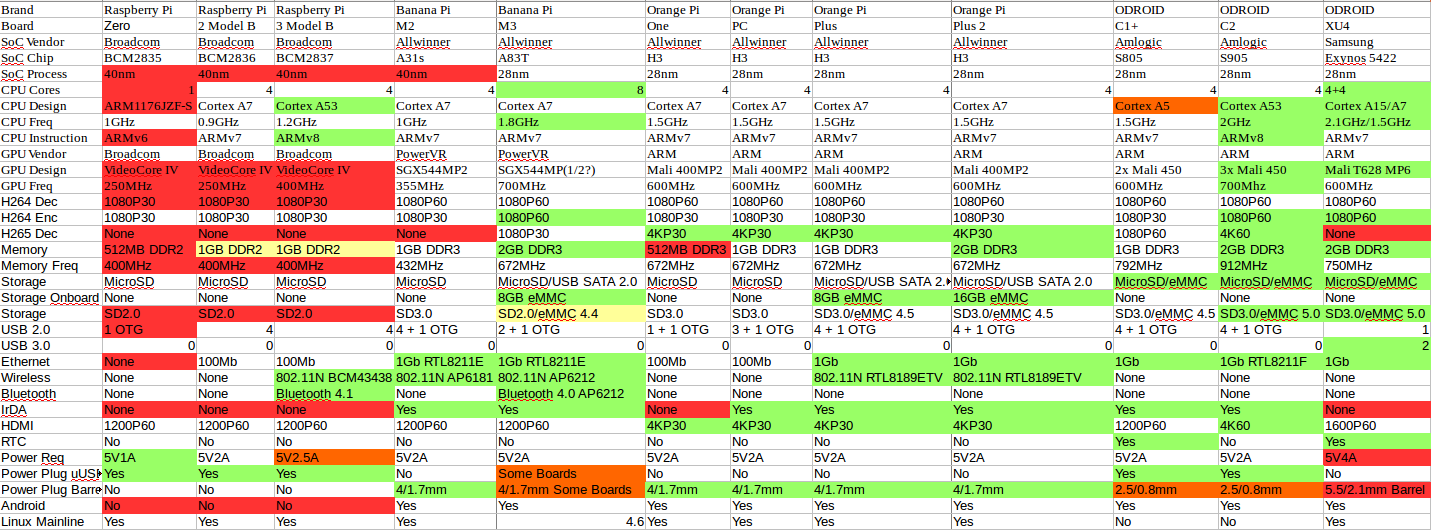
\includegraphics[height=2.5in]{figures/comparativaOrdenadores.png}
\caption[Comparativas de micro-ordenadores]{comparativa de características técnicas de micro-ordenadores\footnotemark}
\end{figure}


Raspberry Pi es posiblemente el uno de los mejores ejemplos de hardware abierto disponibles en el mercado. El diseño de su circuito impreso puede descargarse libremente para crear versiones modificadas.~\cite{raspberry_schematics}. Su precio puede variar notablemente dependiendo del vendedor, pero generalmente no debe superar los 35 euros. Dispone de capacidad suficiente para ejecutar distintos SO basados en arquitectura ARM. En el capitulo siguiente de la propuesta se evaluara que SO utilizar. De entre las distintas opciones disponibles, Raspberry Pi posee una de las comunidades de usuarios mas grandes del mundo, posee una amigable documentación de uso e interminables ejemplos de uso y proyectos disponibles en la red. Sus especificaciones técnicas son suficientes para sostener los servicios necesarios para un prototipo de suite domotica, y puede alimentarse con una toma de USB de 5 Voltios.

\begin{figure}[hbt!]
\centering
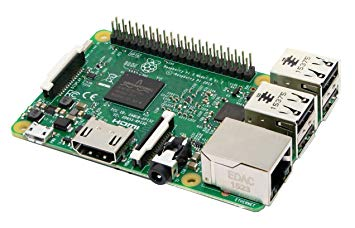
\includegraphics[height=2.5in]{figures/raspberrypi3b.jpg}
\caption[captura de una Raspberry]{Ordenador Raspberry Pi 3B\footnotemark}
\end{figure}

\vspace{1.5cm}


Esto cubriría el soporte físico necesario para crear un gateway. Pero por si solo no es suficiente. Los dispositivos que conectaremos a esta solución pueden presentarse en distintas opciones de hardware que pueden operar entre si y con el propio gateway mediante conectividad \gsl{wifi}. Gracias a los protocolos de comunicación disponibles, un gateway puede comunicarse con dispositivos de distintos fabricantes, presentando en la aplicación a todos ellos como dispositivos homogéneos con diferentes funciones.

\vspace{1.5cm}

En esencia, la clasificación de actores que conforman la red domótica se dividen en el gateway (aunque pueden existir varios), los sensores y los actuadores. De hecho, un actuador no esta restringido a actuar también como sensor y viceversa. Esta clasificación responde a la facilidad de entender rápidamente si un dispositivo actúa como entrada o salida del sistema. En \gls{iot} es habitual disponer de hardware especializado de bajo consumo y orientado a protocolo concretos de comunicación para ser usados en frameworks, como ocurre con OpenHab, que hace facilita bastante la tarea de incluir nuevos dispositivos a la suite domótica si el producto a  integrar ya esta implementado. Si se desea disponer de la flexibilidad de cambiar radicalmente el comportamiento  de un actor, modificando su comportamiento y hardware, es mejor plantear el uso de placas microcontroladoras programables.

\vspace{1.5cm}

Estas placas, al no estar sujetos a un implementación y diseño cerrados, pueden cambiar y ajustarse a nuevos comportamientos y especificaciones, lo cual aportan mayor escalabilidad y facilita la capacidad de actualizar el código programado. Por contrapartida, al ser de uso genérico, su consumo eléctrico para operar es mayor que en los dispositivos diseñados específicamente para una tarea concreta. Es sin embargo, una limitación aceptable, ya que el prototipo busca la funcionalidad sobre el rendimiento.

\vspace{1.5cm}

Uno de los ejemplos mas conocidos y amigables de usar en placas micro-controladoras programables es Arduino. Estas placas disponen de conexiones \gls{io} que pueden usarse para ampliar su abanico e capacidades técnicas, en prototipos de \gls{iot}, es habitual dotar a una placa con conectividad \gls{wifi} mediante un adaptador inalámbrico conocido como shield.

\vspace{1.5cm}

En los últimos años ha aparecido un pequeño microcontrolador con chip de \gls{wifi} conocido generalmente como modulo ESP-01. Este chip permite una comunicación con el protocolo TCP/IP en una red inalámbrica. Se clasifica como hardware RF/IF y RFID CI de transceptor RF, capaz de operar con el protocolo 802.11b/g/n  de 2.4GHz. El modelo ESP8266 que actualmente se comercializa posee capacidades superiores a su predecesora ESP8265 incluye una mayor capacidad de memoria flash interna, suficiente para abordar la mayoría de dispositivos \gls{iot} que pretendan actuar como actuadores o sensores.
Sin embargo, trabajar y programar estos chips puede resultar engorroso si no se dispone de USB con interfaz para escritura en serie, también puede hacerse con una placa de Arduino separando la cucaracha del microcontrolador del Aurdino y cableando la conexión necesaria para programarse desde un ordenador. 

\begin{figure}[hbt!]
\centering
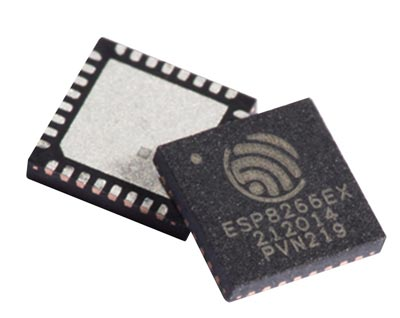
\includegraphics[height=2.5in]{figures/esp8266ex.jpg}
\caption[controladora ESP8233]{controladora ESP8266\footnotemark}
\end{figure}

\vspace{1.5cm}

Este microcontrolador opera con apenas 3.3VDC, lo cual es considerado como una ventaja a la hora de incluir este modulo en proyectos que operan sobre otras placas micro-controladoras como Arduino. Sin embargo, esta opción es valida solo para la creación de prototipos funcionales, ya que el modulo ESP-01 requiere de un amperaje de al menos 200mAh para operar con normalidad. Los pines de alimentación de 3,3V de placas como Arduino ofrecen unos 50mAh de intensidad de corriente. Esto es suficiente para que el modulo opere, pero ocasionalmente puede causar daños en el modulo y generalmente el funcionamiento de la conexión es de baja calidad, con poca intensidad de señal, perdidas de paquetes y caídas de la conexión. La estrategia mas extendida en facilitar una conexión estable de alimentación al modulo separado de la alimentación recibida por la placa microcontroladora en la que opera.

\vspace{1.5cm}

También pueden ejecutarse construcciones simples en una breadboard para un divisor de potencia mediante resistencias que transforme la señal de 5V de las placas microcontroladores, que habitualmente ofrecen un mayor valor de amperios, para dar una señal de 3.3VDC con mas de 200mAh. Siendo realistas, no es ni si quera necesario crearlos si se considera las opciones de venta de algunos fabricantes que montan una microcontrolador con chip ESP8266 en una ensamblada con las resistencias necesarias, interruptores y habitualmente sensores o actuadores como el mostrado en la imagen siguiente\footnotetext{ESP-01S con relé} a modo de modulo compacto alimentado por pines a 5V. El precio de estos módulos apenas alcanza un par de euros si se solicita a vendedores chinos, pero, es conveniente entender los riesgos que se asume al adquirir estos dispositivos de fabricantes clónicos con dudosos controles de calidad, que pueden seleccionar componentes incompatibles son redes \gls{wifi} como el suministrado por el adaptador inalámbrico de una Respaberry Pi 3B. Mas información sobre estos problemas están ampliados en anexo B de trobuleshoting.

\begin{figure}[hbt!]
\centering
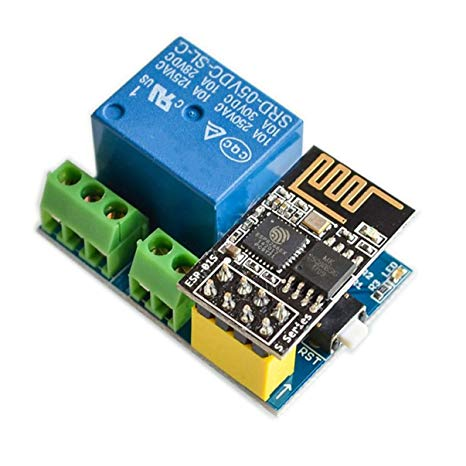
\includegraphics[height=2.5in]{figures/esp8266exRele.jpg}
\caption[ESP-01S con rele]{ESP8266 5V Modulo Rele\footnotemark}
\end{figure}

\vspace{1.5cm}

Con las complicaciones de alimentación del modulo ESP8266 surge al poco tiempo su sucesor natural, las placas nodeMCU. Conocidas pos ser plataformas de código abierto para \gls{iot} mas versátiles y accesibles en coste de adquisición. Uno de los aspectos que popularizo estos dispositivos fue la posterior portabilidad de la biblioteca de MQTT, permitiendo  al LUA de la SOC desplegar dicho protocolo. Aunque el proyecto de mantenimiento de firmware fue abandonado en 2015 por los autores originales, la comunidad de usuarios siguió mejorando el código hasta fecha de hoy, convirtiendo el nodeMCU en uno de los dispositivos mas demandados en proyectos, gracias a su bajo coste de precio, inferior a una decena de euros por placa, que dispone de 12 pines de GPIO permitiendo implementaciones complejas que aprovechan la conectividad inalámbricas para proyectos de \gls{iot}

\begin{figure}[hbt!]
\centering
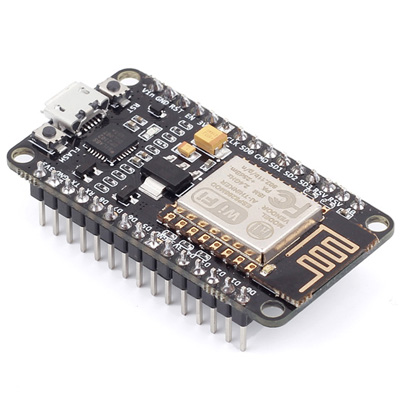
\includegraphics[height=2.5in]{figures/nodemcu.jpg}
\caption[captura de una nodeMCU]{Microcontroladora NodeMCU\footnotemark}
\end{figure}

